\documentclass[10pt]{beamer}
\usepackage[utf8]{inputenc}
\usepackage{tikz, pgfplots}
\pgfplotsset{compat=1.18}
\usetikzlibrary{positioning}
\usetikzlibrary{trees}
\usetikzlibrary{shapes.geometric, arrows.meta, positioning}
\usepackage{xcolor}
\usepackage{graphicx}
\usepackage{subcaption}
\usepackage{hyperref} 
\usepackage{colortbl} % Required for \rowcolor
\usepackage{animate}
\usepackage[T1]{fontenc}
\usepackage{amsmath, amsfonts, amssymb}
\usepackage{cancel}
\usepackage[french]{babel}
\usepackage[normalem]{ulem}
\usepackage{multicol}

\setlength{\columnsep}{1cm}        % khoảng cách giữa 2 cột
\setlength{\columnseprule}{2pt}    % độ rộng vạch đứng
\renewcommand{\columnseprulecolor}{\color{gray}} % màu vạch

% Theme và màu sắc cho beamer
\usetheme{AnnArbor}
\usecolortheme{seahorse}

% Định nghĩa và thiết lập màu sắc chung
\definecolor{mydarkblue}{RGB}{0,51,102}
\setbeamercolor{structure}{fg=mydarkblue}
\setbeamercolor{frametitle}{bg=mydarkblue, fg=white}
\setbeamercolor{title}{fg=mydarkblue}
\setbeamercolor{item}{fg=mydarkblue}
\setbeamercolor{block title}{bg=mydarkblue, fg=white}
\setbeamercolor{block body}{bg=white, fg=black}
\setbeamercolor{section in toc}{fg=mydarkblue}
\setbeamercolor{subsection in toc}{fg=mydarkblue}
\setbeamercolor{caption name}{fg=mydarkblue}
\setbeamercolor{author}{fg=mydarkblue}
\setbeamercolor{date}{fg=mydarkblue}
\setbeamercolor{institute}{fg=mydarkblue}
\setbeamertemplate{caption}[numbered]
\usepackage{multirow}
\title{Rapport Hebdo}
\author{Viet Anh Quach}
\institute{3SR}
\date{\today}

\begin{document}

% \begin{frame}
%     \titlepage
% \end{frame}

\section{Étude bibliographie}

\section{DEM}

% 03102025
\begin{frame}{Article Stress-strain behavior of sand at high strain rates (Mehdi Omidvar et al,2012)}
            \begin{figure}[h]
                \centering
                \scalebox{0.4}{\includegraphics{StrainRate.png}}
            \end{figure}
            "Under HSR loading, there is not enough time for strain energy
accumulation, which prohibits crushing and promotes
rolling-rearrangement resulting in a higher resistance to shear"
\end{frame}


\begin{frame}{Trouver le régime de l'état critique}
    \begin{columns}
                \begin{column}{0.5\textwidth}
            \begin{figure}
                \centering
                \scalebox{0.5}{% GNUPLOT: LaTeX picture with Postscript
\begingroup
  \makeatletter
  \providecommand\color[2][]{%
    \GenericError{(gnuplot) \space\space\space\@spaces}{%
      Package color not loaded in conjunction with
      terminal option `colourtext'%
    }{See the gnuplot documentation for explanation.%
    }{Either use 'blacktext' in gnuplot or load the package
      color.sty in LaTeX.}%
    \renewcommand\color[2][]{}%
  }%
  \providecommand\includegraphics[2][]{%
    \GenericError{(gnuplot) \space\space\space\@spaces}{%
      Package graphicx or graphics not loaded%
    }{See the gnuplot documentation for explanation.%
    }{The gnuplot epslatex terminal needs graphicx.sty or graphics.sty.}%
    \renewcommand\includegraphics[2][]{}%
  }%
  \providecommand\rotatebox[2]{#2}%
  \@ifundefined{ifGPcolor}{%
    \newif\ifGPcolor
    \GPcolortrue
  }{}%
  \@ifundefined{ifGPblacktext}{%
    \newif\ifGPblacktext
    \GPblacktextfalse
  }{}%
  % define a \g@addto@macro without @ in the name:
  \let\gplgaddtomacro\g@addto@macro
  % define empty templates for all commands taking text:
  \gdef\gplbacktext{}%
  \gdef\gplfronttext{}%
  \makeatother
  \ifGPblacktext
    % no textcolor at all
    \def\colorrgb#1{}%
    \def\colorgray#1{}%
  \else
    % gray or color?
    \ifGPcolor
      \def\colorrgb#1{\color[rgb]{#1}}%
      \def\colorgray#1{\color[gray]{#1}}%
      \expandafter\def\csname LTw\endcsname{\color{white}}%
      \expandafter\def\csname LTb\endcsname{\color{black}}%
      \expandafter\def\csname LTa\endcsname{\color{black}}%
      \expandafter\def\csname LT0\endcsname{\color[rgb]{1,0,0}}%
      \expandafter\def\csname LT1\endcsname{\color[rgb]{0,1,0}}%
      \expandafter\def\csname LT2\endcsname{\color[rgb]{0,0,1}}%
      \expandafter\def\csname LT3\endcsname{\color[rgb]{1,0,1}}%
      \expandafter\def\csname LT4\endcsname{\color[rgb]{0,1,1}}%
      \expandafter\def\csname LT5\endcsname{\color[rgb]{1,1,0}}%
      \expandafter\def\csname LT6\endcsname{\color[rgb]{0,0,0}}%
      \expandafter\def\csname LT7\endcsname{\color[rgb]{1,0.3,0}}%
      \expandafter\def\csname LT8\endcsname{\color[rgb]{0.5,0.5,0.5}}%
    \else
      % gray
      \def\colorrgb#1{\color{black}}%
      \def\colorgray#1{\color[gray]{#1}}%
      \expandafter\def\csname LTw\endcsname{\color{white}}%
      \expandafter\def\csname LTb\endcsname{\color{black}}%
      \expandafter\def\csname LTa\endcsname{\color{black}}%
      \expandafter\def\csname LT0\endcsname{\color{black}}%
      \expandafter\def\csname LT1\endcsname{\color{black}}%
      \expandafter\def\csname LT2\endcsname{\color{black}}%
      \expandafter\def\csname LT3\endcsname{\color{black}}%
      \expandafter\def\csname LT4\endcsname{\color{black}}%
      \expandafter\def\csname LT5\endcsname{\color{black}}%
      \expandafter\def\csname LT6\endcsname{\color{black}}%
      \expandafter\def\csname LT7\endcsname{\color{black}}%
      \expandafter\def\csname LT8\endcsname{\color{black}}%
    \fi
  \fi
    \setlength{\unitlength}{0.0500bp}%
    \ifx\gptboxheight\undefined%
      \newlength{\gptboxheight}%
      \newlength{\gptboxwidth}%
      \newsavebox{\gptboxtext}%
    \fi%
    \setlength{\fboxrule}{0.5pt}%
    \setlength{\fboxsep}{1pt}%
    \definecolor{tbcol}{rgb}{1,1,1}%
\begin{picture}(7200.00,5040.00)%
    \gplgaddtomacro\gplbacktext{%
      \csname LTb\endcsname%%
      \put(682,704){\makebox(0,0)[r]{\strut{}$-5$}}%
      \csname LTb\endcsname%%
      \put(682,1527){\makebox(0,0)[r]{\strut{}$0$}}%
      \csname LTb\endcsname%%
      \put(682,2350){\makebox(0,0)[r]{\strut{}$5$}}%
      \csname LTb\endcsname%%
      \put(682,3173){\makebox(0,0)[r]{\strut{}$10$}}%
      \csname LTb\endcsname%%
      \put(682,3996){\makebox(0,0)[r]{\strut{}$15$}}%
      \csname LTb\endcsname%%
      \put(682,4819){\makebox(0,0)[r]{\strut{}$20$}}%
      \csname LTb\endcsname%%
      \put(814,484){\makebox(0,0){\strut{}$0$}}%
      \csname LTb\endcsname%%
      \put(1469,484){\makebox(0,0){\strut{}$5$}}%
      \csname LTb\endcsname%%
      \put(2124,484){\makebox(0,0){\strut{}$10$}}%
      \csname LTb\endcsname%%
      \put(2779,484){\makebox(0,0){\strut{}$15$}}%
      \csname LTb\endcsname%%
      \put(3435,484){\makebox(0,0){\strut{}$20$}}%
      \csname LTb\endcsname%%
      \put(4090,484){\makebox(0,0){\strut{}$25$}}%
      \csname LTb\endcsname%%
      \put(4745,484){\makebox(0,0){\strut{}$30$}}%
      \csname LTb\endcsname%%
      \put(5400,484){\makebox(0,0){\strut{}$35$}}%
      \csname LTb\endcsname%%
      \put(6055,484){\makebox(0,0){\strut{}$40$}}%
      \put(6187,704){\makebox(0,0)[l]{\strut{}$-5$}}%
      \put(6187,1527){\makebox(0,0)[l]{\strut{}$0$}}%
      \put(6187,2350){\makebox(0,0)[l]{\strut{}$5$}}%
      \put(6187,3173){\makebox(0,0)[l]{\strut{}$10$}}%
      \put(6187,3996){\makebox(0,0)[l]{\strut{}$15$}}%
      \put(6187,4819){\makebox(0,0)[l]{\strut{}$20$}}%
      \put(1862,4325){\makebox(0,0)[r]{\strut{}hpd}}%
      \put(1862,4161){\makebox(0,0)[r]{\strut{}gd}}%
    }%
    \gplgaddtomacro\gplfronttext{%
      \csname LTb\endcsname%%
      \put(209,2761){\rotatebox{-270}{\makebox(0,0){\strut{}$\varepsilon_{v}(hpd) (\%)$}}}%
      \put(6693,2761){\rotatebox{-270}{\makebox(0,0){\strut{}$\varepsilon_{v}(gd) (\%)$}}}%
      \put(3434,154){\makebox(0,0){\strut{}$\varepsilon_{yy} (\%)$}}%
    }%
    \gplbacktext
    \put(0,0){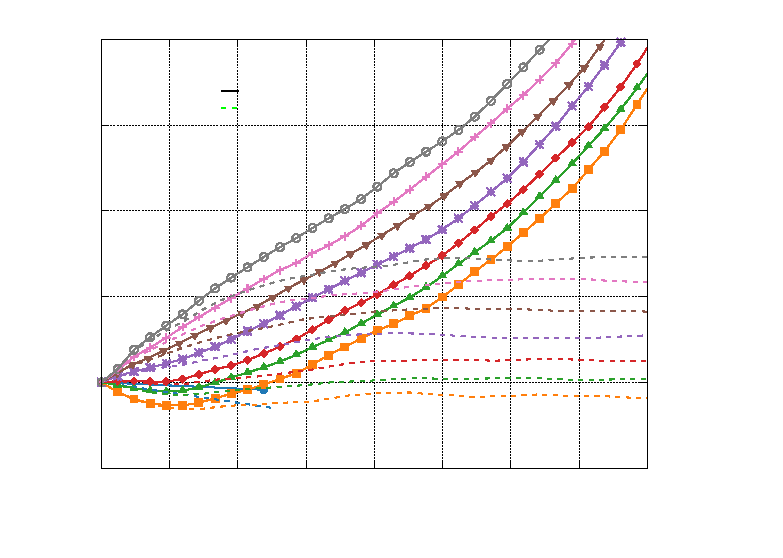
\includegraphics[width={360.00bp},height={252.00bp}]{Eyy_Ev}}%
    \gplfronttext
  \end{picture}%
\endgroup
}
                \caption{Déformation Volumique}
            \end{figure}
            \small
            hpp: $\varepsilon_{yy} = \dfrac{\Delta h_{yy}}{h_{yy}^0}; \varepsilon_v = \varepsilon_{xx} + \varepsilon_{yy} + \varepsilon_{zz} $\\
            gd: $\varepsilon_{yy} = \ln\left(\dfrac{h_{yy}}{h_{yy}^0}\right);  \varepsilon_v = \dfrac{\Delta V}{V_0}$;
        \end{column}
        \begin{column}{0.5\textwidth}
            \begin{figure}
                \centering
                \scalebox{0.5}{\input{NombreCoordination.tex}}
                \caption{Nombre de Coordination}
            \end{figure}
            $Z = \dfrac{2N_{contact}}{N_{particule}}$; $I = \dfrac{v}{H_0}\sqrt{\dfrac{m}{P\overline{a}}}$
        \end{column}
    \end{columns}
\end{frame}

\begin{frame}{Trouver le régime de l'état critique}
    \begin{columns}
                \begin{column}{0.5\textwidth}
            \begin{figure}
                \centering
                \scalebox{0.5}{\input{Aleatoire.tex}}
                \caption{Nombre de Coordination}
            \end{figure}
            échantillon aléatoire par compression dans l'axe Z
        \end{column}
        \begin{column}{0.5\textwidth}
            \begin{figure}
                \centering
                \scalebox{0.5}{\input{ComparerNP.tex}}
                \caption{Nombre de Particules}
            \end{figure}
        \end{column}
    \end{columns}

\end{frame}


\section{MPM}
\begin{frame}{État Rankine - Modèle}
            \begin{figure}
                \centering
                  \includegraphics[height = 2.3cm]{activeRankine.pdf}
                \caption{Pression active}
            \end{figure}       
                        \begin{figure}
                \centering
                  \includegraphics[height = 2.3cm]{passiveRankine.pdf}
                \caption{Pression passive}
            \end{figure}  
        Observer la pression sur le mur en bleu
        \end{frame}


                \begin{frame}{Paramètres principaux}
    \begin{table}
        \centering
        \begin{tabular}{|c|l|l|}
            \hline
                \textbf{Symbole} & \textbf{Paramètre} & \textbf{Valeur} \\
            \hline
            $L$ & Longueur & 3 m \\
            $H$ & Hauteur & 1 m \\
            $\rho$ & Densité & $2700\ \mathrm{kg/m^3}$ \\
            $E$ & Module de Young  & $1\times10^{9}\ \mathrm{Pa}$ \\
            $\nu$ & Coefficient de Poisson  & 0.2 \\
            $\varphi$ & Angle de frottement interne  & $25^{\circ}$\\
            $\psi$ & Angle de dilatance  & $\approx 0^{\circ}$\\
            $v$ & Vélocité de déplacement & 0.005 m/s\\
            $c$ & Cohésion & 0 \& 100 Pa\\
            $\mu$ & \parbox[t]{4.5cm}{Coefficient de frottement entre\\ le mur et les PMs\\} & 0 \& 0\\
            \hline
        \end{tabular}
        \caption{Paramètres du modèle (loi Mohr-Coulomb)}
    \end{table}
\end{frame}

\begin{frame}{État Rankine - Stabiliser}
    \begin{multicols}{2}
            \begin{figure}
                \centering
                \includegraphics[height = 4cm]{pressureEnBas.png}
                \caption{Pression en bas}
            \end{figure}     
            $P_{\text{théorique}} = 2.65e4\ (Pa) $
            \columnbreak  
            \begin{figure}
                \centering
                \scalebox{0.45}{\input{energieCinetique.tex}}
                \caption{Énergie cinétique}
                $P_{\text{simulation}} = 2e4\ (Pa)$
            \end{figure}
        \end{multicols}
                       \center\textcolor{red}{ $\rightarrow$ L'écart est $0.65$ kPa}
        \end{frame}

\begin{frame}{État Rankine - Théorie}
            Coefficient K: la relation entre la contrainte verticale et horizontal:
            \begin{itemize}
           \item Poussée active: $K_a = \dfrac{1 - \sin(\varphi)}{1 + \sin(\varphi)} = 0.406$\\
\item Poussée passive: $K_p = 1/K_a = 2.464$\\
\item État au repos: $ K_0 = 1 - \sin(\varphi) = 0.577$
            \end{itemize}
La somme de pression $F$(kN) appliqué sur le mur:
\begin{multicols}{2}
\noindent
Sans cohésif: \\
\[
F_a = \dfrac{1}{2}\gamma H^2 K_a = 5.376861
\]
\[
F_a = \dfrac{1}{2}\gamma H^2 K_p = 32.619458
\]
\[
F_0 = \dfrac{1}{2}\gamma H^2 K_0 = 7.647
\]

\columnbreak

\noindent
Cohésif:
\[
F_a = \dfrac{1}{2}\gamma H^2 K_a - 2cH\sqrt{K_a} = 5.249425
\]
\[
F_p = \dfrac{1}{2}\gamma H^2 K_p + 2cH\sqrt{K_p} = 32.93334
\]
\[
F_0 = \dfrac{1}{2}\gamma H^2 K_p + 2cH\sqrt{K_0} = 7.495
\]

\end{multicols}
\end{frame}

        \begin{frame}{État Rankine reposé}
            \begin{figure}
                \centering
                \scalebox{0.7}{\input{Repose.tex}}
                \caption{Pression sur le mur en bleu}
               \textcolor{red}{ $\rightarrow$ L'écart est $1$ kPa}
            \end{figure}
        \end{frame}

\begin{frame}{État Rankine - Pression Active}
    \begin{multicols}{2}
            \begin{figure}
                \centering
                  \scalebox{0.45}{\input{ActiveCohesion.tex}}
                \caption{Pression active $v=0.005=const$}
            \end{figure}      
            \columnbreak  
                        \begin{figure}
                \centering
                  \scalebox{0.45}{\input{ActiveVitess.tex}}
                \caption{Pression active $c=0=const$}
                            Effet cinétique?
            \end{figure}  
        \end{multicols}
                               \center\textcolor{red}{ $\rightarrow$ L'écart est $0.65$ kPa}
        \end{frame}

        \begin{frame}{État Rankine - Pression Passive}
    \begin{multicols}{2}
     \begin{figure}
                \centering
                \scalebox{0.45}{\input{PassiveCohesion.tex}}
                \caption{Pression passive $v=-0.005=const$}
            \end{figure}
            \columnbreak  
            \begin{figure}
                \centering
                \scalebox{0.45}{\input{PassiveVitess.tex}}
                \caption{Pression passive $c=0=const$}
                            Effet cinétique?
            \end{figure}
        \end{multicols}
                               \center\textcolor{red}{ $\rightarrow$ L'écart est $1$ kPa}
        \end{frame}
\section{MPM-DEM}



\end{document}
